\section{EVALUATION OF THE IMPLEMENTATION}

\subsection{Methodology}

To evaluate the effectiveness of the implemented educational website on Open Badges, and draw actionable conclusions for future studies and improvements to make, a structured methodology was adopted that combined quantitative performance tracking with qualitative user feedback. 
The aim was to assess not only how well users performed but also how they experienced the site’s content, structure, and gamification features. 

\subsubsection{Data Collection Sources}
The evaluation was based on two core data streams:
\begin{enumerate}
    \item \textbf{Task Interaction Data:} Each user completed five sequential interactive tasks, designed to progressively introduce the key concepts behind Open Badges. 
    Every answer and completion interaction was tracked to log the following data points:
    \begin{itemize}
        \item Correct and Incorrect answer counts.
        \item Time of each answer.
    \end{itemize}
    \item \textbf{Post-Session Survey:} After completing the tasks, users were prompted to complete a structured survey comprising 8 statements for numeric answers and a set of required and optional questions with written answers. 
    Ratings were on a 4-point Likert scale (1 = strongly disagree, 4 = strongly agree). 
    This forced users to pick a stance that would not be neutral. 
    The questions were grouped into three thematic categories:
    \begin{itemize}
        \item \textbf{Gamification}: Measured the motivational effectiveness of game-like elements.
        \item \textbf{Enjoyment}: Assessed user experience and interface satisfaction.
        \item \textbf{Understanding}: Evaluated perceived learning and badge comprehension.
    \end{itemize}
\end{enumerate}

The survey questions with numeric answers were the following:

\begin{itemize}
        \item The interactive tasks made the learning experience more engaging.
        \item The score system engaged me to learn more.
        \item Receiving a badge at the end felt like a meaningful reward.
        \item Was the website enjoyable to use overall?
        \item The website was easy to navigate and worked well on my device.
        \item I would recommend this site to someone interested in learning about Open Badges.
        \item I better understand the concept of Open Badges after completing this website.
        \item I understand what the issued badge represents and how it could be used.
\end{itemize}

Below is the list of written feedback questions that the participants also had the option to or had to leave, which was collected to supplement quantitative findings.
\begin{itemize}
        \item Which task or activity did you find the most useful or engaging for understanding Open Badges? Why?
        \item Which task or activity was the least helpful or enjoyable? Why?
        \item Did the interactive elements ever confuse or distract you from the learning content?
        \item If you answered "Yes" in the previous question, please describe what confused or distracted you, and why.
        \item Did the progression system (unlocking sections as you go) help or hinder your learning experience?
\end{itemize}

The final number of participants in the data collection is 9.

\subsubsection{Technical Stack and Tooling}

All data processing, analysis and visualisations were carried out using Python. 
It provides a transparent and reproducible environment for chart generation, computing statistical summaries, and running statistical tests. 
The Python technical stack includes:
\begin{itemize}
        \item Data manipulation via pandas,
        \item Plotting via matplotlib,
        \item Statistical analysis with scipy.stats.
\end{itemize}

To assess internal consistency within the survey categories, the following statistical analysis tools are used:
\begin{itemize}
        \item \textbf{Cronbach’s alpha}
        \item \textbf{Pearson's correlations}
        \item \textbf{Paired t-test}
\end{itemize}

Open-ended responses from participants were reviewed manually and grouped into common themes.

Finally, the count of participants is 10. 
Importantly, due to certain technical errors related to the backend service provider, some quantitative data was corrupted, and in turn, only 9 participants' data was used, with some tests having to reduce the total count to 7, due to missing or corrupt data.
The survey also had a small technical issue due to which 1 participant's results were incomplete, which led to the total number of survey responses being 9. 
All data remained anonymous throughout the process; therefore, it was not feasible to trace the recipients for resubmission.
The total samples are slightly under the anticipated data, therefore, all data is subject to significant bias.

\subsection{Analysis and Overview}

\subsubsection{Task-Level Performance Analysis}

The evaluation began with a breakdown of user performance across the five core tasks using summary statistics from Table \ref{tab:task_summary_vertical} and complementary visualisations.
Several patterns emerged:
\begin{itemize}
        \item Task 4 stands out with perfect accuracy (1.00) and the lowest average time (2.43s). 
        Notably, this task is made without a possibility to fail, and as such, the task is performed to expectations by all users.
        \item In contrast, Task 3 was the most challenging:
        \begin{itemize}
            \item It had the lowest accuracy (mean = 0.51),
            \item The highest average time per task (42.09s),
            \item And a notably high incorrect-to-correct ratio, as seen in Figure \ref{fig:corr_incorr}\footnote{The table displays the average correct and incorrect answers by all users. All users had to answer all of the questions correctly, so the average correct answers is static across all attempts.}. 
            The task was unique in the way that the users were able to fail twice before discovering the correct answer, if attempted way to complete it was to guess the answer. 
            This made it the most punishing task, suggesting cognitive overload or design ambiguity that warrants a review of either instructional clarity or task mechanics. 
            \begin{figure}[hbtp]
        \centering
        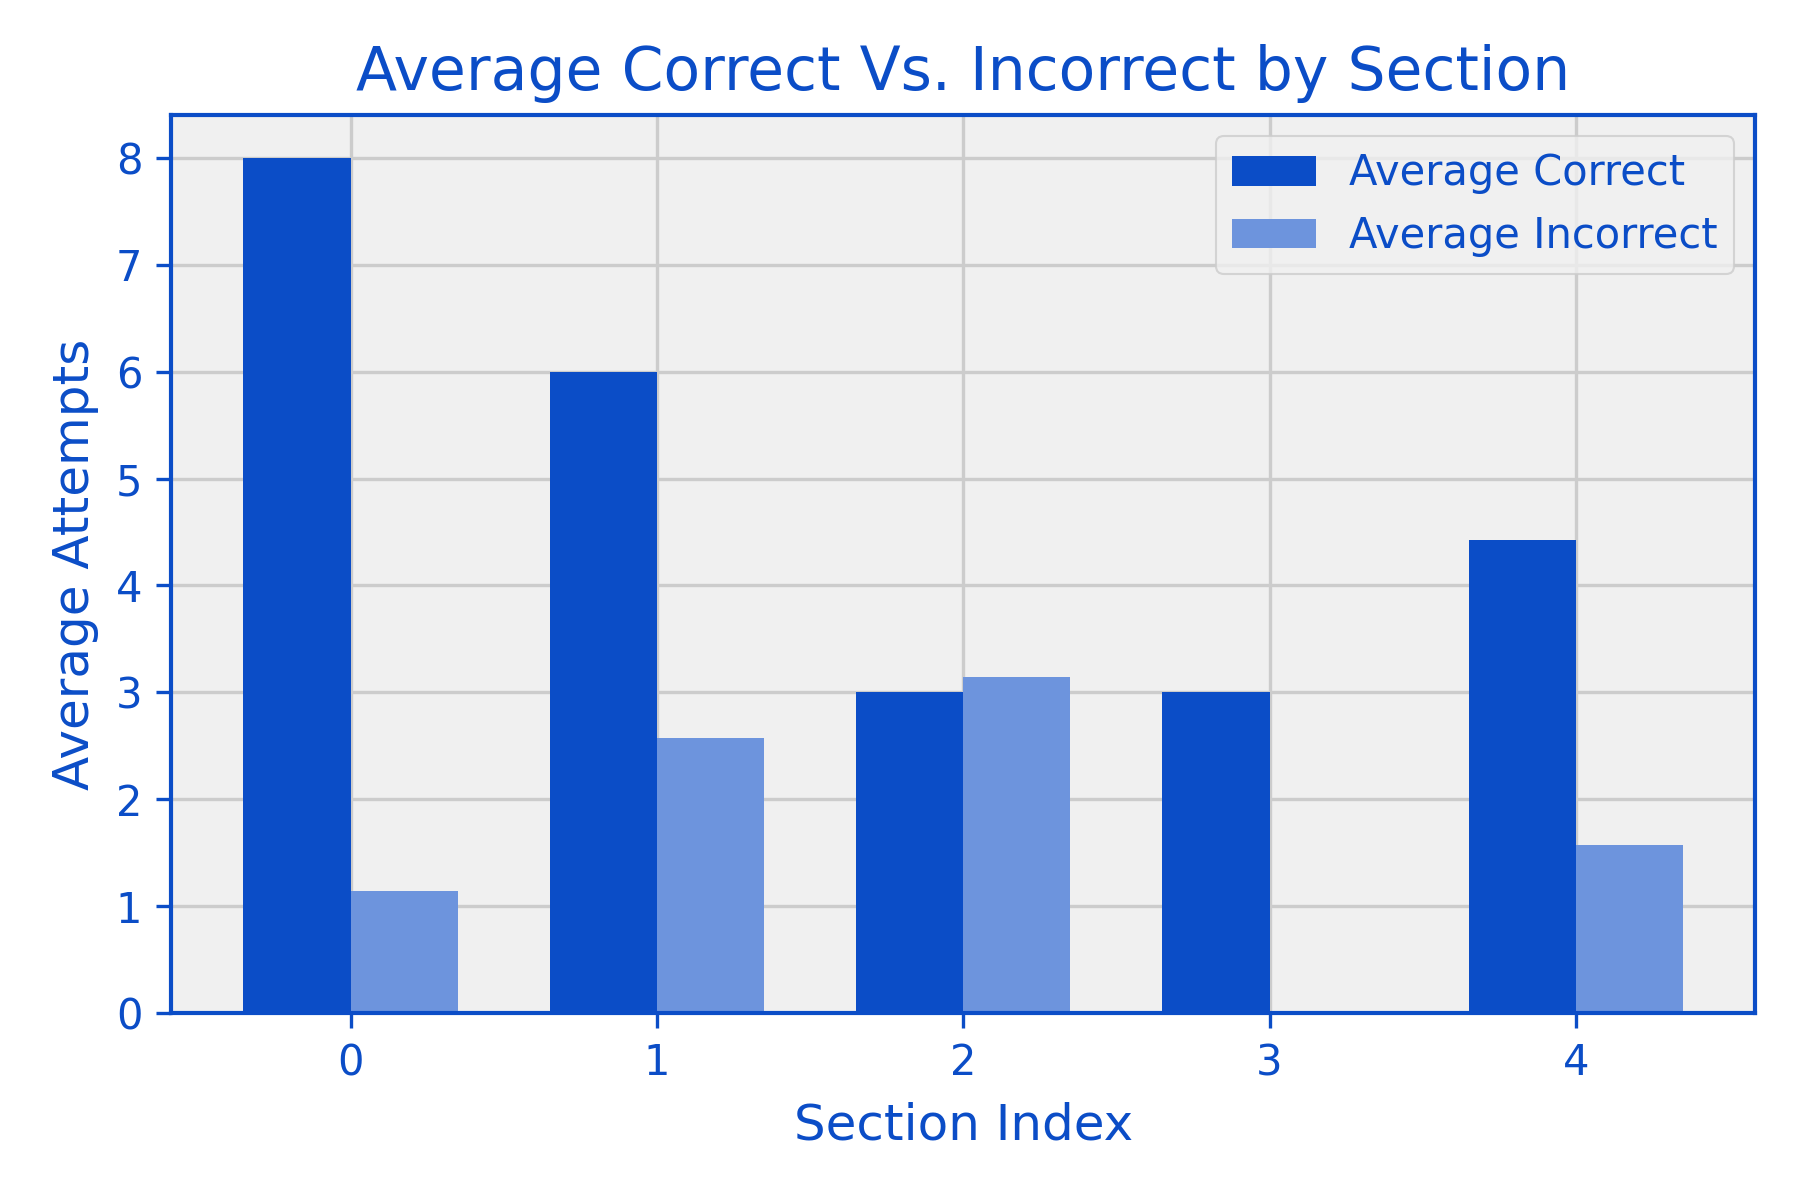
\includegraphics[width=0.8\textwidth]{figures/mean_correct_incorrect.png}
        \caption{Average Correct Vs Incorrect answer aggregations per task by all users}
        \label{fig:corr_incorr}
        {\raggedright \small{Source: created by the author based on project data}\par}
\end{figure}
            \item This is corroborated by the written responses regarding the questions within the task being slightly too vague, which caused mild frustration to users. 
            \item This is further supported by Figure \ref{fig:acc}, where the task, while it has the longest average time per attempt, also holds the lowest accuracy. 
            This implies that additional time in this task did not yield better outcomes.
        \end{itemize}
        \item Tasks 1 and 2 showed intermediate difficulty, with Task 1 offering higher accuracy and slightly longer average time. 
        Task 2 showed many more incorrect attempts on average than Task 1. 
        Notably, Task 1 handles a very familiar topic to most people ("hard" and "soft" skills), in comparison to Task 2, which is about metadata. 
        \item Task 5 showed moderate difficulty but high variance, particularly in accuracy (SD = 0.17) and time (SD = 12.77s), suggesting inconsistent user experience, meaning some people found it easier than others.
        \item Overall, average time per task and accuracy display an upward trend across most tasks, as seen in Figure \ref{fig:acc}.
\end{itemize}

\begin{table}[ht]
\centering
\captionsetup{justification=raggedright, singlelinecheck=false}
\caption{Task-level summary statistics}
\begin{tabular}{lccccc}
\toprule
\textbf{Metric} & \textbf{Task 1} & \textbf{Task 2} & \textbf{Task 3} & \textbf{Task 4} & \textbf{Task 5} \\
\midrule
Avg. Incorrect     & 1.142857 & 2.571429 & 3.142857 & 0.000000 & 1.571429 \\
Avg. Total Attempts& 9.142857 & 8.571429 & 6.142857 & 3.000000 & 7.890000 \\
Avg. Accuracy      & 0.884848 & 0.719048 & 0.511735 & 1.000000 & 0.765136 \\
Std. Accuracy      & 0.098825 & 0.138253 & 0.127387 & 0.000000 & 0.168197 \\
Avg. Time (s)      & 23.556714 & 33.274714 & 42.090000 & 2.430857 & 24.135286 \\
Std. Time (s)      & 8.549135 & 29.238296 & 39.153163 & 0.981814 & 12.770451 \\
\bottomrule
\end{tabular}
\label{tab:task_summary_vertical}
\end{table}
{\raggedright \small{Source: based on results from author's implementation}\par}
\begin{flushleft}
\textsuperscript{†}\textit{Note: All tasks required users to eventually select the correct answer before they could proceed. The "Avg. Total Attempts" metric reflects total interactions needed to reach completion, which may exceed the number of correct options in each task. For example, Task 1 had 8 cards to sort, but users averaged 9.14 attempts. The minimums were 8, 6, 3, 3 and 6 respectively for each task. Therefore, "Accuracy" here represents a ratio of correct responses to total attempts, not a pass/fail score.}
\end{flushleft}


\begin{figure}[hbtp]
\centering
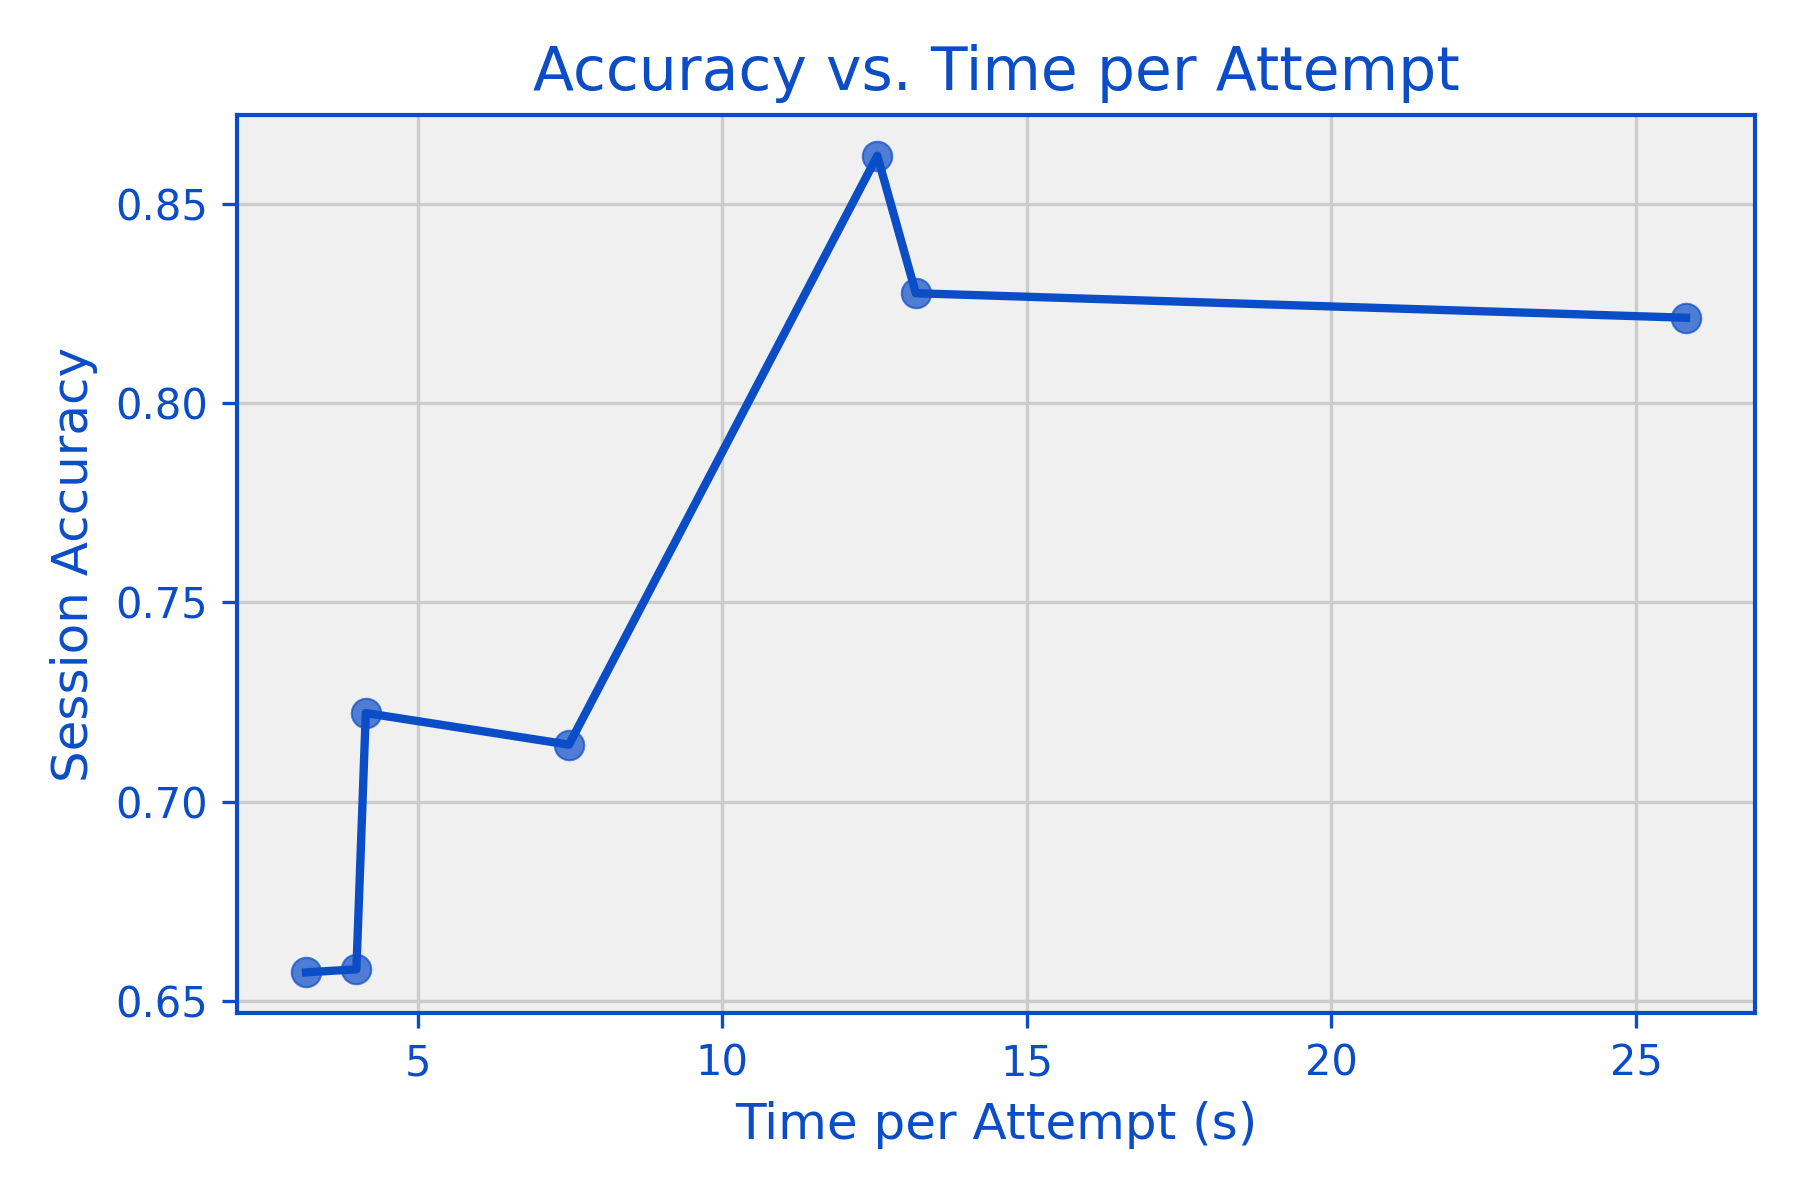
\includegraphics[width=0.8\textwidth]{figures/accuracy_vs_time.png}
\caption{Accuracy Vs Time per Attempt}
\label{fig:acc}
{\raggedright \small{Source: created by the author based on project data}\par}
\end{figure}

The heatmaps further supported these interpretations, showing clear visual hotspots in Task 3 for both extended durations and low accuracy. 
In Figure \ref{fig:acc_hm} tasks 1, 2 and 5 all have reasonable and preferable performance at 0.88 for a great starting performance, followed by a drop for increased challenge and ending with a slight recovery towards the end with Task 5.
Task 4 remains unique and Task 3 continues to stand out as a consistently failed task. 
This reinforces the need to refine its instructions, potentially implement a feedback loop, and rewrite the question prompts for the user to have improved clarity.

\begin{figure}[hbtp]
\centering
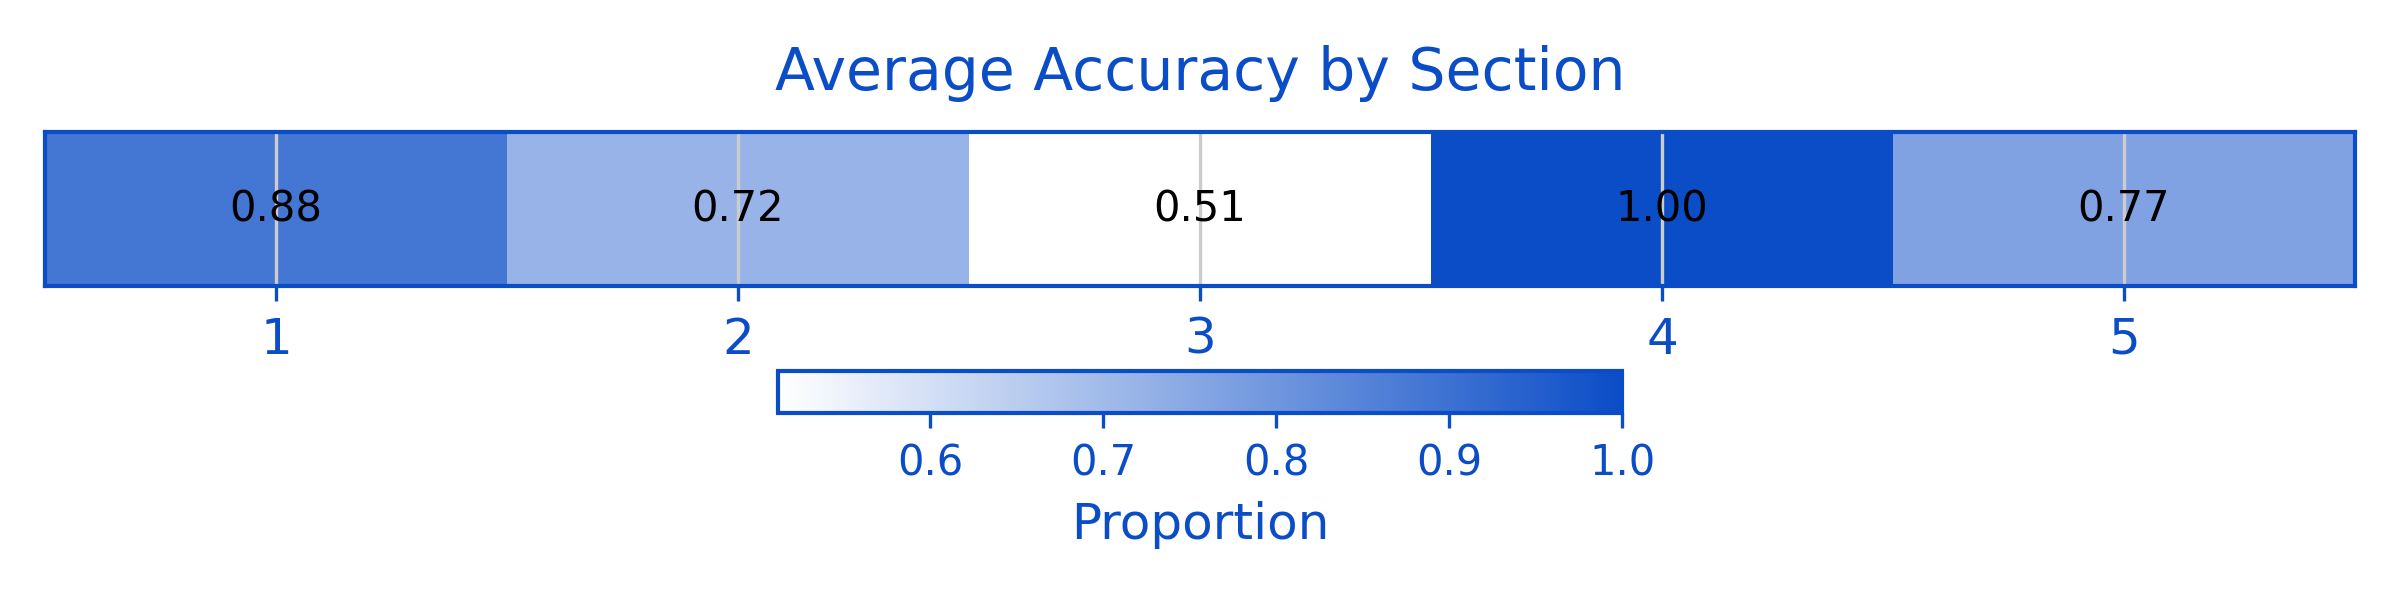
\includegraphics[width=0.8\textwidth]{figures/heatmap_accuracy.png}
\caption{Average Correctness Accuracy per task}
\label{fig:acc_hm}
{\raggedright \small{Source: created by the author based on project data}\par}
\end{figure}

The final heatmap from Figure \ref{fig:q_hm} shows the average time spent per question in each task. 
Task 3 clearly required more thinking with an average of 7.6 seconds but again did not lead to much improved results. 
Tasks 2 and 5 are roughly similar in time required for completion, which is a moderate challenge. 
Task 1 was twice as quick to complete per question in comparison, and with more questions, or rather cards to sort, serves more as a quick-fire intro to settle people in with the interactivity of the website.

\begin{figure}[hbtp]
\centering
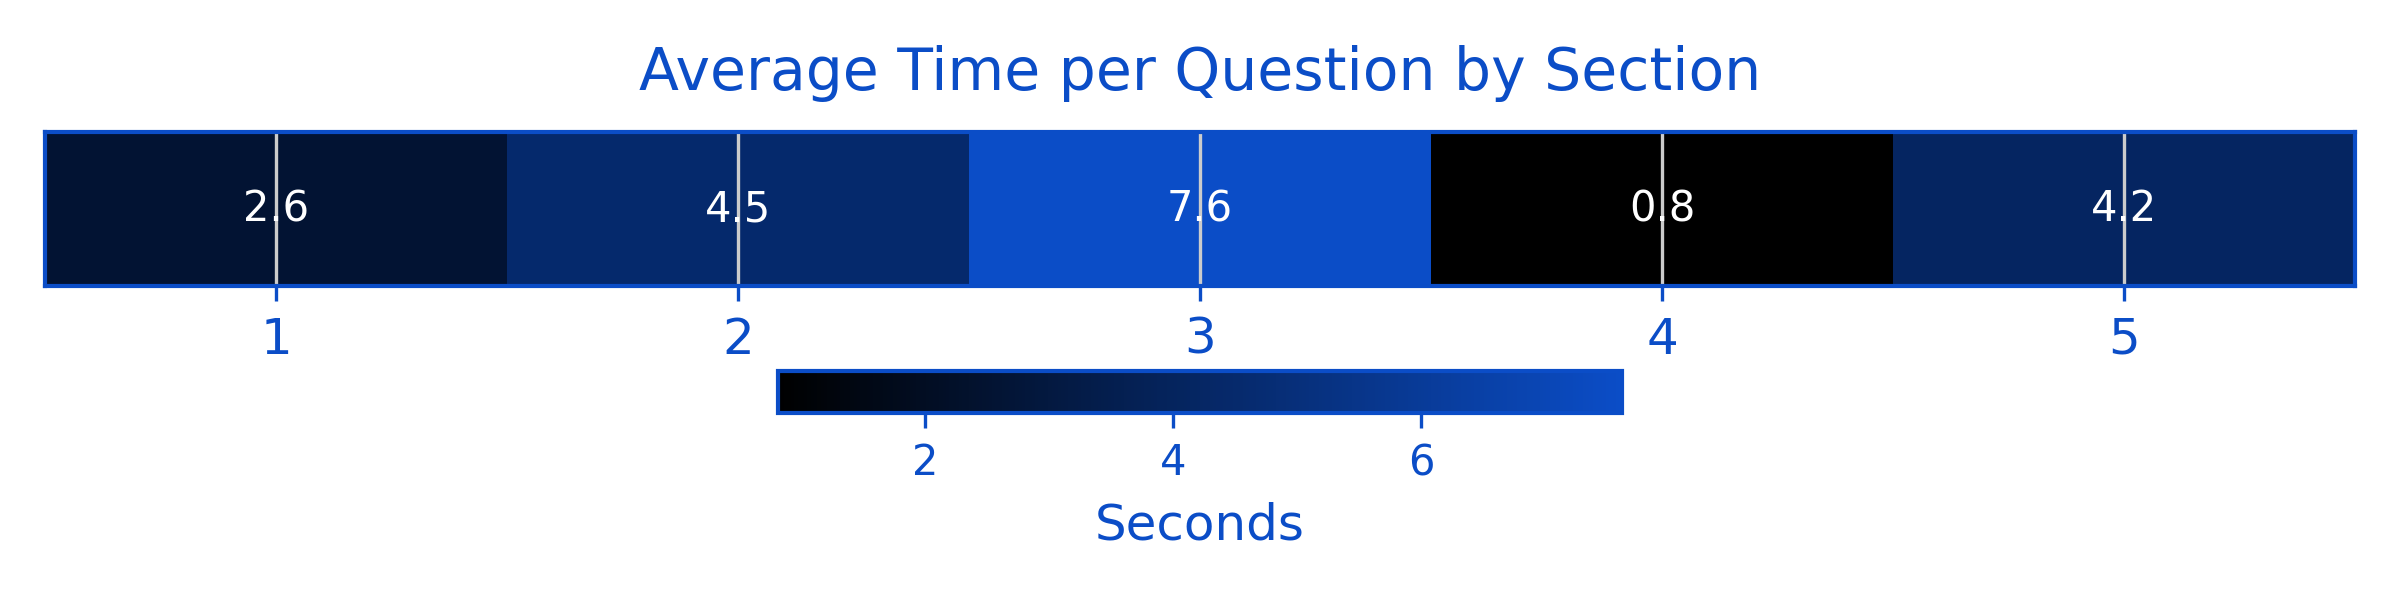
\includegraphics[width=0.8\textwidth]{figures/heatmap_time_per_q.png}
\caption{Average Time per Question by task}
\label{fig:q_hm}
{\raggedright \small{Source: created by the author based on project data}\par}
\end{figure}

\subsubsection{Survey Analysis}

The survey post-completion provided insights into user perception of gamification, enjoyment, and conceptual understanding. 
The numeric results of which can be seen within Table \ref{tab:survey_stats}. 
It has to be reiterated that the respondents were able to select answers between 1 and 4.
Overall sentiment was positive, but differences between categories and within questions revealed some minor insights:

\begin{itemize}
        \item Understanding received the highest ratings, with most users strongly agreeing they now understand Open Badges and their meaning, with mean scores of 3.78 and 3.56, respectively. 
        This confirms that the core educational objective was met successfully.
        \item Enjoyment scores were also consistently high, particularly for the overall website experience, with a mean of 3.67. 
        Navigation and interface satisfaction were likewise strong, with relatively low standard deviation, indicating consistent user satisfaction.
        \item Gamification results were mixed. The highest-rated statement was about interactive tasks enhancing engagement with a mean of 3.56. 
        The lowest result was from the question of whether the badge is a meaningful reward, which scored a mean of 2.89. 
        This disparity was statistically tested using a paired t-test, which returned a non-significant result p = 0.282, suggesting no strong divergence in user sentiment but rather mild skepticism toward the end reward's impact. 
        This is likely due to the certain stigma attached to all badges inherently, which the website is meant to reduce.
\end{itemize}

The correlation matrix further revealed a moderate positive association with a coefficient of 0.47 between Gamification and Enjoyment, indicating that users who felt engaged by the gamified elements also tended to enjoy the platform overall. However, this was not strong enough to claim a causal link.

Internal consistency analysis using Cronbach’s alpha returned:

0.71 for Gamification — acceptable and suggesting a coherent perception among the related items,

0.61 for Enjoyment — borderline, but interpretable, especially with the small sample size.

\begin{table}[ht]
{\small
\centering
\captionsetup{justification=raggedright, singlelinecheck=false}
\caption{Descriptive statistics of survey results}
\label{tab:survey_stats}
\begin{tabular}{|p{4.5cm}|c|c|c|c|c|}
\hline
\textbf{Statement} & \textbf{Category} & \textbf{Mean} & \textbf{SD} & \textbf{Min--Max} & \textbf{r with Enjoyment} \\
\hline
The interactive tasks made the learning experience more engaging. & Gamification & 3.56 & 0.53 & 3--4 & -0.16 \\
\hline
The score system engaged me to learn more. & Gamification & 3.22 & 0.83 & 2--4 & 0.20 \\
\hline
Receiving a badge at the end felt like a meaningful reward. & Gamification & 2.89 & 0.78 & 2--4 & -0.11 \\
\hline
Was the website enjoyable to use overall? & Enjoyment & 3.67 & 0.50 & 3--4 & \textemdash \\
\hline
The website was easy to navigate and worked well on my device. & Enjoyment & 3.44 & 0.53 & 3--4 & 0.16 \\
\hline
I would recommend this site to someone interested in learning about Open Badges. & Enjoyment & 3.44 & 0.73 & 2--4 & 0.46 \\
\hline
I better understand the concept of Open Badges after completing this website. & Understanding & 3.78 & 0.44 & 3--4 & -0.38 \\
\hline
I understand what the issued badge represents and how it could be used. & Understanding & 3.56 & 0.73 & 2--4 & -0.11 \\
\hline
\end{tabular}
}
\end{table}
{\raggedright \small{Source: based on results from author's implementation}\par}

\subsubsection{Qualitative Feedback Themes}
\begin{itemize}
    \item The general sentiment was that Task 1 was the favourite, due to being "Simple but effective" and particularly clear.
    \item In terms of difficulty, Task 3 was mentioned as the least favourable task due to a lack of clarity, increased failure and therefore, unfair loss of points.
    \item Over 80\% of respondents claim that interactive elements did not confuse or distract from the learning experience, and exclusively improved it. Notably, a comment that did describe distraction states that the distraction is rather an incite for the user to learn more and be more attentive rather than confusing.
    \item No respondents stated that the point scoring system hindered the user, some users stated that it had no impact, and the majority stated that it helped their performance.
    \item Within the freeform comment section, a couple of comments were made regarding niche mobile displays having minor visual issues. 
    Additionally, a user stated that the metaphorical "magic" in each step of the website is much appreciated.
\end{itemize}

\subsection{Analysis Conclusions}

The evaluation demonstrates that the implemented educational website effectively achieved its primary objective: helping users understand the core concepts of Open Badges. 
Quantitative data confirms that most tasks were performed with reasonable accuracy, and the post-survey results show a high level of user satisfaction and self-reported learning.

Task-level analysis identified Task 3 as a pain point for users. 
It had the lowest accuracy and highest time of completion, signalling a need for restructuring. 
Conversely, Task 4 was completed consistently completed quickly and flawlessly, due to an entirely different approach of being a leisurely activity in the middle of the user's journey.
Task 1 was praised both qualitatively and quantitatively for its clarity and relevance.

The survey results indicate strong user enjoyment and solid perceived learning outcomes. 
While gamification features were generally well received, the final badge reward was met with some scepticism, possibly due to broader perceptions of badge value. 
The moderate correlation between enjoyment and gamification suggests that while game elements enhanced engagement, they were not the sole driver of satisfaction.

Written feedback supported these conclusions, highlighting both the clarity of earlier tasks and the difficulty of more abstract ones. 
The progression system and interactivity were well received, with no critical usability issues apart from minor display bugs on specific devices.

Despite technical issues that reduced the sample size, the evaluation offers actionable insights: refine vague or overly punishing tasks, increase the reward perception of badges, and preserve what users already find intuitive and engaging. 

\subsection{Limitations and Suggestions for Future Research}

While this evaluation yielded valuable insights, several limitations must be acknowledged that may have affected the generalizability and depth of the findings.

\textbf{1. Small and Partially Corrupted Dataset.}
Due to technical issues with the backend infrastructure, several participant records were either lost or incomplete. 
This significantly reduced statistical power and increased the potential for bias or outlier influence. 
Future research should ensure more robust data integrity mechanisms and aim for a larger, more diverse sample.

\textbf{2. Limited Demographic and Contextual Data.}
No demographic data (e.g., age, digital literacy, or educational background) was collected. 
Such a decision was made due to the small sample size and a biased audience during promotion. 
Primarily, students between the ages of 20 to 30 participated in the data collection. 
As such, it is difficult to assess how prior knowledge or user context influenced learning outcomes or engagement. 
Future studies may benefit from anonymous profiling to better understand how different user types interact with the system.

\textbf{3. Subjective Survey Bias.}
The use of a 4-point Likert scale without a neutral midpoint was intentional to avoid indecision but may have pressured some users into selecting positions that did not fully represent their views. 
Additionally, social desirability bias may have influenced positively skewed responses, especially in small group settings. 
With a larger data sample, the Likert scale could be expanded for greater deviation

\textbf{4. Ambiguity in Task Design.}
The evaluation revealed that Task 3, while well-intentioned, resulted in substantial confusion and disproportionately low scores despite higher effort. 
Future research could be conducted with pilot testing and more rigorous usability reviews of task instructions and mechanics during the design phase.

\textbf{5. Badge Perception Uncertainty.}
Though central to the site's concept, the issued badge was not perceived as strongly meaningful by all users. 
This reflects a broader challenge with Open Badge literacy and acceptance. 
Future work should explore how contextual framing, real-world examples, or even credential-linked integration can enhance the perceived value of the badge system. 

\subsubsection{Recommendations for Future Research:}
\begin{itemize}
\item Recruit a larger and more varied user base to validate performance and perception trends across demographics.
\item Include pre-testing to track changes in user perception of Open Badges and their learning recognition.
\item Experiment with different reward systems or badge types to evaluate what design patterns better convey meaningfulness.
\item Introduce A/B testing for different task versions, e.g., with vs. without feedback or timed vs. untimed, to identify the most effective instructional strategies.
\item Consider longitudinal studies to explore how badge understanding or motivation changes over time.
\item Introduce additional requirements or reward tiers that have to be reached through excellent performance, to obtain the badge, as it is currently given as a participation trophy: everyone is capable of finishing the website regardless of the number of mistakes.
\end{itemize}

By addressing these limitations, future research can build a more complete and nuanced understanding of how gamified learning environments—and Open Badge systems specifically—can best support digital skill recognition and learner engagement.

\newpage